\documentclass[10pt,a4paper,landscape]{article}
% -- Layout ----
\usepackage[top=0.6cm, bottom=0.6cm, left=0.5cm, right=0.5cm, landscape]{geometry}

% -- Titles ----
\usepackage[
  tiny,                     % text size title
  compact                   % reduce vertical space before/after title
]{titlesec}
% \titlespacing*
\titleformat{\section}{\normalfont\small\bfseries}{\thesection}{0em}{} % Remove space before and after section titles
\titleformat{\subsection}{\normalfont\small\bfseries}{\thesubsection}{0em}{} % Remove space before and after subsection titles
\titlespacing*{\section}{0pt}{0pt}{0pt} % Remove space before/after section titles
\titlespacing*{\subsection}{0pt}{0pt}{0pt} % Remove space before/after subsec titles

% -- Colors ----
\usepackage[dvipsnames]{xcolor}
\definecolor{dmm}{RGB}{192,192,192} % Define a custom dimmed text color
\definecolor{cmt}{RGB}{61,123,123}

% -- Math ------
\usepackage{mathtools}
\usepackage{amssymb}
\usepackage{turnstile}%better vdash

% -- Lists -----
\usepackage[inline]{enumitem}
\setlist{noitemsep}% Remove vspace between items
% Set vspace before and after  list environments as well as the left margin
\setlist[itemize,1]{leftmargin=.6em,labelindent=0pt,labelsep=2pt,
  topsep=1pt,partopsep=1pt}
\setlist[enumerate,1]{leftmargin=1em,labelindent=0pt,labelsep=2pt,
  topsep=1pt,partopsep=1pt}
\setlist[itemize,2]{leftmargin=.3em,labelindent=1pt,topsep=1pt,partopsep=1pt}
\setlist[enumerate,2]{leftmargin=0.2em,labelindent=1pt,topsep=1pt,partopsep=1pt}
\setlist[description]{labelwidth=\linewidth,font=\small\bfseries,leftmargin=1em,topsep=1pt,partopsep=1pt}
% -- Code listing ---
\usepackage{listings}
\lstset{
  aboveskip=3pt,
  belowskip=3pt,
  basicstyle=\small\ttfamily,
  breaklines=true,
  % commentstyle=\upshape\ttfamily,
  captionpos=b,
  commentstyle=\color{cmt},
  frame=single,
  keepspaces=false,
  keywordstyle=\bfseries,
  showspaces=false,
  showstringspaces=false,
  showtabs=false,
  tabsize=2,
}

% Parse Trees
\usepackage{tikz}
\usetikzlibrary{ arrows, automata, bbox, calc, positioning,  decorations.pathmorphing, decorations.pathreplacing, decorations.shapes, }
\tikzset{
% ->, % makes the edges directed
>=stealth', % makes the arrow heads bold
node distance=1cm, % specifies minimum distance between two nodes
% small/.style={},
every state/.style={thick}, % sets the properties for each ’state’ node
every node/.style={inner sep=1pt},
initial text=start, % sets the text that appears on the start arrow
}

% Place a figure env right here via [H] option
\usepackage{float}

% Side by side figure
\usepackage{subcaption}
% \usepackage{caption}
% \captionsetup{belowskip=0pt, aboveskip=0pt}


% -- Multi-Col layout --
\usepackage{multicol}

% No indentation
\setlength\parindent{0pt}
\setlength\abovedisplayskip{-5pt}
\setlength\belowdisplayskip{-5pt}
\setlength\abovedisplayshortskip{-4pt}
\setlength\belowdisplayshortskip{-4pt}
\newcommand{\gor}{\;|\;}
\newcommand{\num}{\texttt{\#}~}
\renewcommand{\arraystretch}{1.2}

\begin{document}
\pagestyle{empty}
\begin{multicols*}{3}
\section*{Predictive parsing - LL(1) and its parse table}
\begin{align*}
  E \to\;& E + T \gor T         \tag{1} \\
  T \to\;& T * F \gor F         \tag{2} \\
  F \to\;& (E) \gor \mathsf{id} \tag{3}
\end{align*}
\section*{Step 1: Eliminate left recursion (if any or skip if none)}
\begin{align*}
  E\,  & \to\; TE'                     \tag{1} \\
  E'\, & \to\; +\,TE' \gor \varepsilon \tag{2} \\
  T\,  & \to\; FT'                     \tag{3} \\
  T'\, & \to\; *\,FT' \gor \varepsilon \tag{4} \\
  F\,  & \to\; (E)    \gor \mathsf{id} \tag{5}
\end{align*}
\section*{Step 2: Remove common prefix by left factoring}
\mb{NO} common prefix shared by any 2 productions, so skip

\section*{Step 3: Collect FIRST and FOLLOW sets}
\begin{itemize}
\item \mo{FIRST} set for each production
  \begin{align*}
    \mfn{first}(E)  &= \mfn{first}(T) = \mfn{first}(F) \\
                    &= \mfn{first}(() \cup \mfn{first}(\mathsf{id})
                      = \mset{\left(\right.,\mathsf{id}} \\
    \mfn{first}(E') &= \mfn{first}(+)\cup\mfn{first}(\varepsilon)
                      = \mset{+,\varepsilon}                  \\
    \mfn{first}(T)  &= \mfn{first}(F) = \mset{(,\mathsf{id}}  \\
    \mfn{first}(T') &= \mfn{first}(*)\cup\mfn{first}(\varepsilon)
                      = \mset{*,\varepsilon}  \\
    \mfn{first}(F)  &= \mfn{first}(()\cup\mfn{first}(\mathsf{id})
                      = \mset{(,\mathsf{id}}
  \end{align*}
\item \mo{FOLLOW} set for each production (include \$(\texttt{EOF}))
  \begin{align*}
    \mfn{follow}(E)  &= \mfn{first}()) = \mset{)} \Rightarrow \mset{), \$}     \\
    \mfn{follow}(E') &= \mfn{follow}(E) = \mset{), \$} \Rightarrow \mset{), \$}\\
    \mfn{follow}(T)  &= \mfn{first}(E')\cup\mfn{follow}(E')\cup\mfn{follow(E)} \\
                     &= \mset{+, \left.\right), \$} \\
    \mfn{follow}(T') &= \mfn{follow}(T) = \mset{+, ), \$}\\
    \mfn{follow}(F)  &= \mfn{first}(T')\cup\mfn{follow}(T)= \mset{*, +, ), \$}
    \end{align*}
  \item summary table of \mo{FIRST} and \mo{FOLLOW} sets
    \begin{center}
      \begin{tabular}{l|l|r}
        \hline
        N  & \textsf{FIRST} & \textsf{FOLLOW} \\
        \hline
        \(E\)   & \(\mset{(,\mathsf{id}}\) & \(\mset{), \$}\) \\
        \(E'\)  & \(\mset{+,\varepsilon}\) & \(\mset{), \$}\) \\
        \(T\)   & \(\mset{(,\mathsf{id}}\) & \(\mset{+, ), \$}\) \\
        \(T'\)  & \(\mset{*,\varepsilon}\) & \(\mset{+, ), \$}\) \\
        \(F\)   & \(\mset{(,\mathsf{id}}\) & \(\mset{*, +, ), \$}\) \\
        \hline
      \end{tabular}
  \end{center}
\end{itemize}


\section*{Step 4: LL(1) parse table}
\begin{enumerate}
\item For \mb{non-$\varepsilon$} productions, use \mo{\textsf{FIRST}(RHS)} to locate cols and put production or production number there
  \begin{align*}
    \mfn{first}(RHS_{E}) &=\mfn{first}(TE')=\mfn{first}(T) = \mset{(,\mathsf{id}} \\
    \mfn{first}(RHS_{E'})&=\mfn{first}(+TE')=\mfn{first}(+) = \mset{+} \\
    \mfn{first}(RHS_{T}) &=\mfn{first}(FT')=\mfn{first}(F) = \mset{(,\mathsf{id}} \\
    \mfn{first}(RHS_{T'})&=\mfn{first}(*FT')=\mfn{first}(*) = \mset{*} \\
    \mfn{first}(RHS_{F}) &=\mfn{first}((E))= \mfn{first}(() = \mset{(} \\
    \mfn{first}(RHS_{F}) &=\mfn{first}(\mathsf{id}) = \mset{\mathsf{id}}
  \end{align*}
  \begin{tabular}{l|c|c|c|c|c|c}
  \hline
  N       & +          & id  & *          & (           & )   & \$(\texttt{EOF})\\
  \hline
  \(E\)   &            &\(\to TE'\)&& \(\to TE'\) &     & \\
  \(E'\)  &\(\to +TE'\)& &&&\\
  \(T\)   &            &\(\to FT'\)    &            &\(\to FT'\) &\\
  \(T'\)  &            &      &\(\to *FT'\)&&\\
  \(F\)   &            &\(\to \mathsf{id}\)& &\(\to (E)\)&&\\
  \hline
  \multicolumn{7}{l}{rows: non-terminals (LHS); cols: terminals; entry: RHS}\\
  \hline
  \multicolumn{7}{l}{can also use production number for each entry}\\
  \hline
  \end{tabular}
\vspace{.1em}
\item For \mb{$\boldsymbol{\varepsilon}$} productions, use \mo{\textsf{FOLLOW}(LHS)} to locate cols and put \mb{$\boldsymbol{\varepsilon}$} there
  \begin{align*}
    \mfn{follow}(LHS_{E'})&= \mset{), \$}\\
    \mfn{follow}(LHS_{T'})&= \mset{+, ), \$}
  \end{align*}
  \begin{tabular}{l|c|c|c|c|c|c}
  \hline
  N       & +          & id  & *          & (           & )   & \$(\texttt{EOF})\\
  \hline
  \(E\)   &            &\(\to TE'\)&      & \(\to TE'\) && \\
  \(E'\)  &\(\to +TE'\)&     &            &  &\(\varepsilon\) &\(\varepsilon\)\\
  \(T\)   &            &\(\to FT'\)    &                &\(\to FT'\) &\\
  \(T'\)  &\(\varepsilon\) & &\(\to *FT'\)&  &\(\varepsilon\)&\(\varepsilon\)\\
  \(F\)   &            &\(\to \mathsf{id}\)& &\(\to (E)\)&&\\
  \hline
  \multicolumn{7}{l}{rows: non-terminals (LHS); cols: terminals; entry: RHS}\\
  \hline
  \multicolumn{7}{l}{can also use production number for each entry}\\
  \hline
  \end{tabular}
\end{enumerate}
\begin{itemize}
\item If the grammar includes minus \mb{-}, it will be the same as \mb{+}
\item if the grammar includes division \mb{$\boldsymbol{\backslash}$}, it will be the same as \mb{*}
\item if the grammar includes a start symbol $S\to E\$$
  \begin{center}
  \begin{tabular}{l|l|l}
    \hline
    N      & \textsf{FIRST} & \textsf{FOLLOW} (empty) \\
    \hline
    \(S\)  & \(\mset{(,\mathsf{id}}\) & \\
    \hline
    \multicolumn{3}{l}{FIRST same as $E$, FOLLOW is empty}\\
    \hline
  \end{tabular}\\
  \begin{tabular}{l|c|c|c|c|c|c}
  \hline
  N       & +          & id  & *          & (           & )   & \$(\texttt{EOF})\\
  \hline
  \(S\)   &            &\(\to E\$\)&      & \(\to E\$\) && \\
  \hline
  \end{tabular}
  \end{center}
\end{itemize}
\section*{LL (1) parsing example (suppose stack top is the left end)}
\begin{enumerate}
\item \mb{Update stack} stack top is a non-terminal; try to replace it with RHS of its production(s)
\item \mb{Input match} stack top is terminal; match with current input symbol; remove the symbol from input; pop stack
\item \mb{Accept}: stack = input buffer = \$
\item \mb{Error}: when there is a mismatch, throws error
\end{enumerate}
\begin{minipage}{\linewidth}
\centering
\begin{tabular}{l|l|l|l}
  \hline
  Stack & Input buffer                          & Action  & Use Production  \\
  \hline
  $E\$$ & $\mathsf{id}*\mathsf{id}+\mathsf{id}\$$ & Update stack & $E\to TE'$\\
  $TE'\$$ & $\mathsf{id}*\mathsf{id}+\mathsf{id}\$$ & Update stack &$T\to FT'$\\
  $FT'E'\$$ & $\mathsf{id}*\mathsf{id}+\mathsf{id}\$$ & Update stack$^{\mr{1}}$ &$F\to \mathsf{id}$\\
  $\mathsf{id}T'E'\$$ & $\mathsf{id}*\mathsf{id}+\mathsf{id}\$$ & Match &\\
  $T'E'\$$ & $*\mathsf{id}+\mathsf{id}\$$ & Update stack$^{\mr{2}}$ & $T'\to *FT'$\\
  $*FT'E'\$$ & $*\mathsf{id}+\mathsf{id}\$$ & Match & \\
  $FT'E'\$$ & $\mathsf{id}+\mathsf{id}\$$ & Update stack &$F\to \mathsf{id}$ \\
  $\mathsf{id}T'E'\$$ & $\mathsf{id}+\mathsf{id}\$$ & Match & \\
  $T'E'\$$ & $+\mathsf{id}\$$ & Update stack$^{\mr{3}}$ & $T'\to \varepsilon$\\
  $E'\$$ & $+\mathsf{id}\$$ & Update stack & $E'\to +TE'$\\
  $+TE'\$$ & $+\mathsf{id}\$$ & Match & \\
  $TE'\$$ & $\mathsf{id}\$$ & Update stack & $T\to FT'$\\
  $FT'E'\$$ & $\mathsf{id}\$$ & Update stack & $F\to \mathsf{id}$\\
  $\mathsf{id}T'E'\$$ & $\mathsf{id}\$$ & Match & \\
  $T'E'\$$ & $\$$ & Update stack & $T'\to \varepsilon$ \\
  $E'\$$ & $\$$ & Update stack & $E'\to \varepsilon$ \\
  $\$$ & $\$$ & Accept &  \\
  \hline
  \multicolumn{4}{l}{\mr{1}: LL(1) parser knows $F\to \mathsf{id}$ if it sees \textsf{id} ahead}\\
  \hline
  \multicolumn{4}{l}{\mr{2}: LL(1) parser knows $T'\to *FT'$ if it sees \textsf{*} ahead}\\
  \hline
  \multicolumn{4}{l}{\mr{3}: LL(1) parser knows $T'\to \varepsilon$ if it sees other stuff ahead}\\
  \hline
\end{tabular}
\end{minipage}
\begin{itemize}
\item \textbf{Use Prod.} shows the leftmost derivation and parse tree
  \begin{center}
    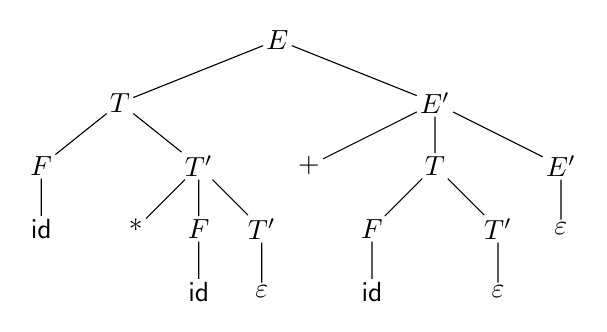
\begin{tikzpicture}[level distance=8mm]
      \node {$E$}
      [sibling distance=40mm]
      child {
        node {$T$}
        [sibling distance=20mm]
        child {
          node {$F$} child { node {\mr{$\mathsf{id}$}} }
        }
        child {
          node {$T'$}
          [sibling distance=8mm]
          child  {node {\mr{*}}}
          child  {node {$F$} child {node {\mr{$\mathsf{id}$}}}}
          child  {node {$T'$} child {node {\mr{$\varepsilon$}}}}
        }
      }
      child {
        node {$E'$}
        [sibling distance=16mm]
        child  {node {\mr{+}}}
        child  {
          node {$T$}
          child {node {$F$} child {node {\mr{$\mathsf{id}$}}}}
          child {node {$T'$} child {node {\mr{$\varepsilon$}}}}
        }
        child  {node {$E'$} child {node {\mr{$\varepsilon$}}}}
      };
    \end{tikzpicture}
    \end{center}
\item leaf nodes from left to right build the original input string
\[\mathsf{id} * \mathsf{id} + \mathsf{id} \]
\end{itemize}


\section*{LL (1) parsing example (suppose stack top is the left end)}
\begin{enumerate}
\item \mb{Update stack} stack top is a non-terminal; try to replace it with RHS of its production(s)
\item \mb{Input match} stack top is terminal; match with current input symbol; remove the symbol from input; pop stack
\item \mb{Accept}: stack = input buffer = \$
\item \mb{Error}: when there is a mismatch, throws error
\end{enumerate}
\begin{minipage}{\linewidth}
\centering
\begin{tabular}{l|l|l|l}
  \hline
  Stack & Input buffer                          & Action  & Use Production  \\
  \hline
  $E\$$ & $\mathsf{id}*\mathsf{id}+\mathsf{id}\$$ & Update stack & $E\to TE'$\\
  $TE'\$$ & $\mathsf{id}*\mathsf{id}+\mathsf{id}\$$ & Update stack &$T\to FT'$\\
  $FT'E'\$$ & $\mathsf{id}*\mathsf{id}+\mathsf{id}\$$ & Update stack$^{\mr{1}}$ &$F\to \mathsf{id}$\\
  $\mathsf{id}T'E'\$$ & $\mathsf{id}*\mathsf{id}+\mathsf{id}\$$ & Match &\\
  $T'E'\$$ & $*\mathsf{id}+\mathsf{id}\$$ & Update stack$^{\mr{2}}$ & $T'\to *FT'$\\
  $*FT'E'\$$ & $*\mathsf{id}+\mathsf{id}\$$ & Match & \\
  $FT'E'\$$ & $\mathsf{id}+\mathsf{id}\$$ & Update stack &$F\to \mathsf{id}$ \\
  $\mathsf{id}T'E'\$$ & $\mathsf{id}+\mathsf{id}\$$ & Match & \\
  $T'E'\$$ & $+\mathsf{id}\$$ & Update stack$^{\mr{3}}$ & $T'\to \varepsilon$\\
  $E'\$$ & $+\mathsf{id}\$$ & Update stack & $E'\to +TE'$\\
  $+TE'\$$ & $+\mathsf{id}\$$ & Match & \\
  $TE'\$$ & $\mathsf{id}\$$ & Update stack & $T\to FT'$\\
  $FT'E'\$$ & $\mathsf{id}\$$ & Update stack & $F\to \mathsf{id}$\\
  $\mathsf{id}T'E'\$$ & $\mathsf{id}\$$ & Match & \\
  $T'E'\$$ & $\$$ & Update stack & $T'\to \varepsilon$ \\
  $E'\$$ & $\$$ & Update stack & $E'\to \varepsilon$ \\
  $\$$ & $\$$ & Accept &  \\
  \hline
  \multicolumn{4}{l}{\mr{1}: LL(1) parser knows $F\to \mathsf{id}$ if it sees \textsf{id} ahead}\\
  \hline
  \multicolumn{4}{l}{\mr{2}: LL(1) parser knows $T'\to *FT'$ if it sees \textsf{*} ahead}\\
  \hline
  \multicolumn{4}{l}{\mr{3}: LL(1) parser knows $T'\to \varepsilon$ if it sees other stuff ahead}\\
  \hline
\end{tabular}
\end{minipage}
\begin{itemize}
\item \textbf{Use Prod.} shows the leftmost derivation and parse tree
  \begin{center}
    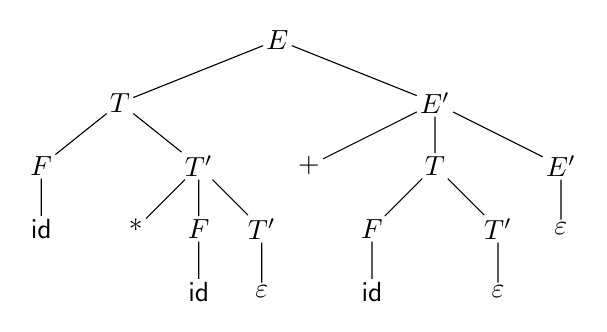
\begin{tikzpicture}[level distance=8mm]
      \node {$E$}
      [sibling distance=40mm]
      child {
        node {$T$}
        [sibling distance=20mm]
        child {
          node {$F$} child { node {\mr{$\mathsf{id}$}} }
        }
        child {
          node {$T'$}
          [sibling distance=8mm]
          child  {node {\mr{*}}}
          child  {node {$F$} child {node {\mr{$\mathsf{id}$}}}}
          child  {node {$T'$} child {node {\mr{$\varepsilon$}}}}
        }
      }
      child {
        node {$E'$}
        [sibling distance=16mm]
        child  {node {\mr{+}}}
        child  {
          node {$T$}
          child {node {$F$} child {node {\mr{$\mathsf{id}$}}}}
          child {node {$T'$} child {node {\mr{$\varepsilon$}}}}
        }
        child  {node {$E'$} child {node {\mr{$\varepsilon$}}}}
      };
    \end{tikzpicture}
    \end{center}
\item leaf nodes from left to right build the original input string
\[\mathsf{id} * \mathsf{id} + \mathsf{id} \]
\end{itemize}

\end{multicols*}
\end{document}
